% 2006_liaoning_liberal_q19_fig1: left unfolded square + right folded solid (two panels)
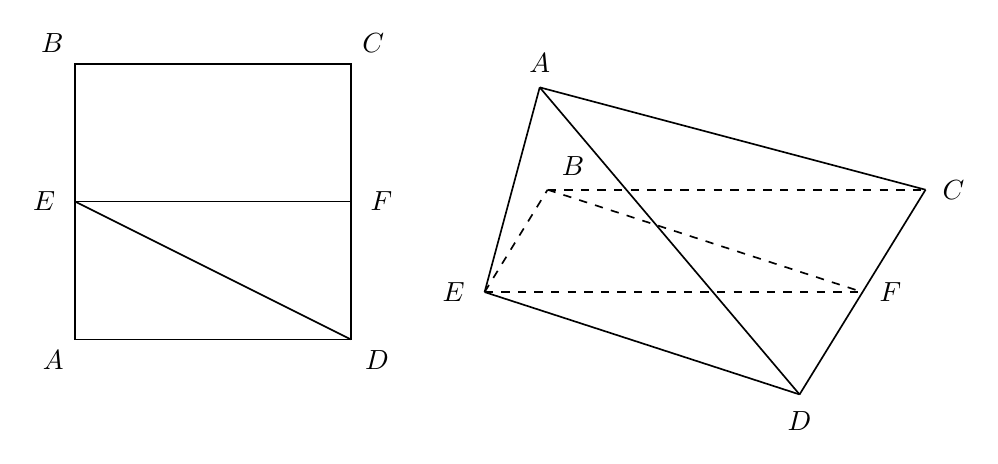
\begin{tikzpicture}[x=1cm,y=1cm,font=\normalsize,
  geometry edge/.style={solid,line width=.6pt},
  geometry label/.style={font=\normalsize,inner sep=2pt}]
% ---- left panel: square B-C-D-A, midline E-F, diagonal E-D ----
\coordinate (lB) at (-6.5,2.0);
\coordinate (lC) at (-3.0,2.0);
\coordinate (lD) at (-3.0,-1.5);
\coordinate (lA) at (-6.5,-1.5);
\coordinate (lE) at (-6.5,0.25);
\coordinate (lF) at (-3.0,0.25);
\draw[geometry edge] (lB)--(lC)--(lD)--(lA)--cycle;
\draw[geometry edge] (lE)--(lF);
\draw[geometry edge] (lE)--(lD);
\node[geometry label,above left] at (lB) [xshift=-2pt,yshift=2pt] {$B$};
\node[geometry label,above right] at (lC) [xshift=2pt,yshift=2pt] {$C$};
\node[geometry label,below right] at (lD) [xshift=3pt,yshift=-2pt] {$D$};
\node[geometry label,below left] at (lA) [xshift=-2pt,yshift=-2pt] {$A$};
\node[geometry label,left] at (lE) [xshift=-5pt] {$E$};
\node[geometry label,right] at (lF) [xshift=5pt] {$F$};
% ---- right panel: folded body ----
\coordinate (A) at (-0.6000000000,1.7000000000);
\coordinate (E) at (-1.3000000000,-0.9000000000);
\coordinate (D) at (2.7000000000,-2.2000000000);
\coordinate (F) at (3.5000000000,-0.9000000000);
\coordinate (C) at (4.3000000000,0.4000000000);
\coordinate (B) at (-0.5000000000,0.4000000000);
% solid edges
\draw[geometry edge] (E)--(A);
\draw[geometry edge] (A)--(C);
\draw[geometry edge] (A)--(D);
\draw[geometry edge] (E)--(D);
\draw[geometry edge] (D)--(F);
\draw[geometry edge] (F)--(C);
% hidden edges (dashed)
\draw[geometry edge,dashed] (E)--(B);
\draw[geometry edge,dashed] (B)--(C);
\draw[geometry edge,dashed] (B)--(F);
\draw[geometry edge,dashed] (E)--(F);
\node[geometry label,above] at (A) [yshift=3pt] {$A$};
\node[geometry label,left] at (E) [xshift=-5pt] {$E$};
\node[geometry label,below] at (D) [yshift=-4pt] {$D$};
\node[geometry label,right] at (F) [xshift=4pt] {$F$};
\node[geometry label,right] at (C) [xshift=4pt] {$C$};
\node[geometry label,above right=3pt] at (B) {$B$};
\end{tikzpicture}
